\documentclass[../rapport_MVEX01-11-05]{subfiles}
\begin{document}

\section{Implementering av HMM för klassificering av icke-statiska gester}
För att klassificera dynamiska gester bygger man vidare på den metod som användes
för de statiska.  HMM kräver att gester utgörs av följder av symboler,
motsvarande olika observationer. Dessa symboler får vi från en 
klassificering med \knn, med en prototypmängd enligt nedan.
Idén är att representera varje gest, statisk som dynamisk, i form av en
symbolföljd.  De statiska definieras lättast som två eller tre efterföljande
symboler av samma typ, medan de dynamiska består av en följd av blandade
symboler.

Eftersom de statiska gesterna redan tilldelats
symboler är svårigheten att tilldela dynamiska gester symboler på ett effektivt sätt. Vår tanke
är att dela upp filmerna med dynamiska gester i tre kategorier: prototypfilmer, träningsfilmer och 
testfilmer. Tilldelningen av symboler sker genom att varje prototypfilm
delas upp i fyra lika långa delar. Den 
första fjärdedelen tilldelas en symbol, den andra en annan o.s.v.
Förhoppningen är att det som ligger i en viss fjärdedel alltid motsvarar samma
del av gesten, eftersom de tilldelas samma symbol.
De symboler som förknippats med dessa delgester, används med
tillhörande egenskapsvektorer för att definiera nya klasser i prototypmängden.

Programmet omvandlar därefter träningsfilmerna till symboler med \knn i
prototypmängden.
Längden av 
symbolföljden för respektive gest beror på programmets prestanda, d.v.s. hur många bilder 
man önskar analysera per sekund. Det bör uppmärksammas att varianter av en och
samma gest,
beroende på dess längd, kommer att representeras av olika långa symbolföljder,
vilket leder till att vi tränar flera HMM-modeller för varje gest.
En möjlighet är att gruppera symbolsekvenserna 
i tre längder för att motverka alltför strikta krav på gestens utförande. 

HMM-modellerna tränas med Baum-Welch-metoden via \MATLAB-funktionen \texttt{hmmtrain}.
Vi använder Bakis-modellen då den enligt kapitel \ref{sec:hmmtypes}
ger bra resultat i samband med signaler som förändras över tid.
Den är en typ av HMM som medför att
modellerna måste tränas med flera symbolsekvenser \cite{Rabiner89}.
Då ingen förflyttning till ett tidigare
tillstånd är tillåten blir modellen mycket selektiv när det gäller
vilka symboler varje tillstånd kan generera. 
Att endast använda en symbolföljd skulle träna modellen till att systematiskt
vandra från ett tillstånd till nästa,
och i varje tillstånd generera rätt symbol i ordningen med sannolikhet ett.
\notes{tydligt nog?}

För att beräkna sannolikheten för att en viss HMM har skapat en
symbolföljd används \MATLAB-funktionen \texttt{hmmviterbi}. 
Om vi antar att det har tränats HMM-modeller för gester av längd två,
fem och sju symboler, kommer programmets klassificering 
av testfilmerna att ske på det sätt som beskrivs i
figur~\vref{fig:hmm-flowchart}.
 
 \begin{figure}[tbp]
  \centering
  \captionsetup{singlelinecheck=off} % hack
  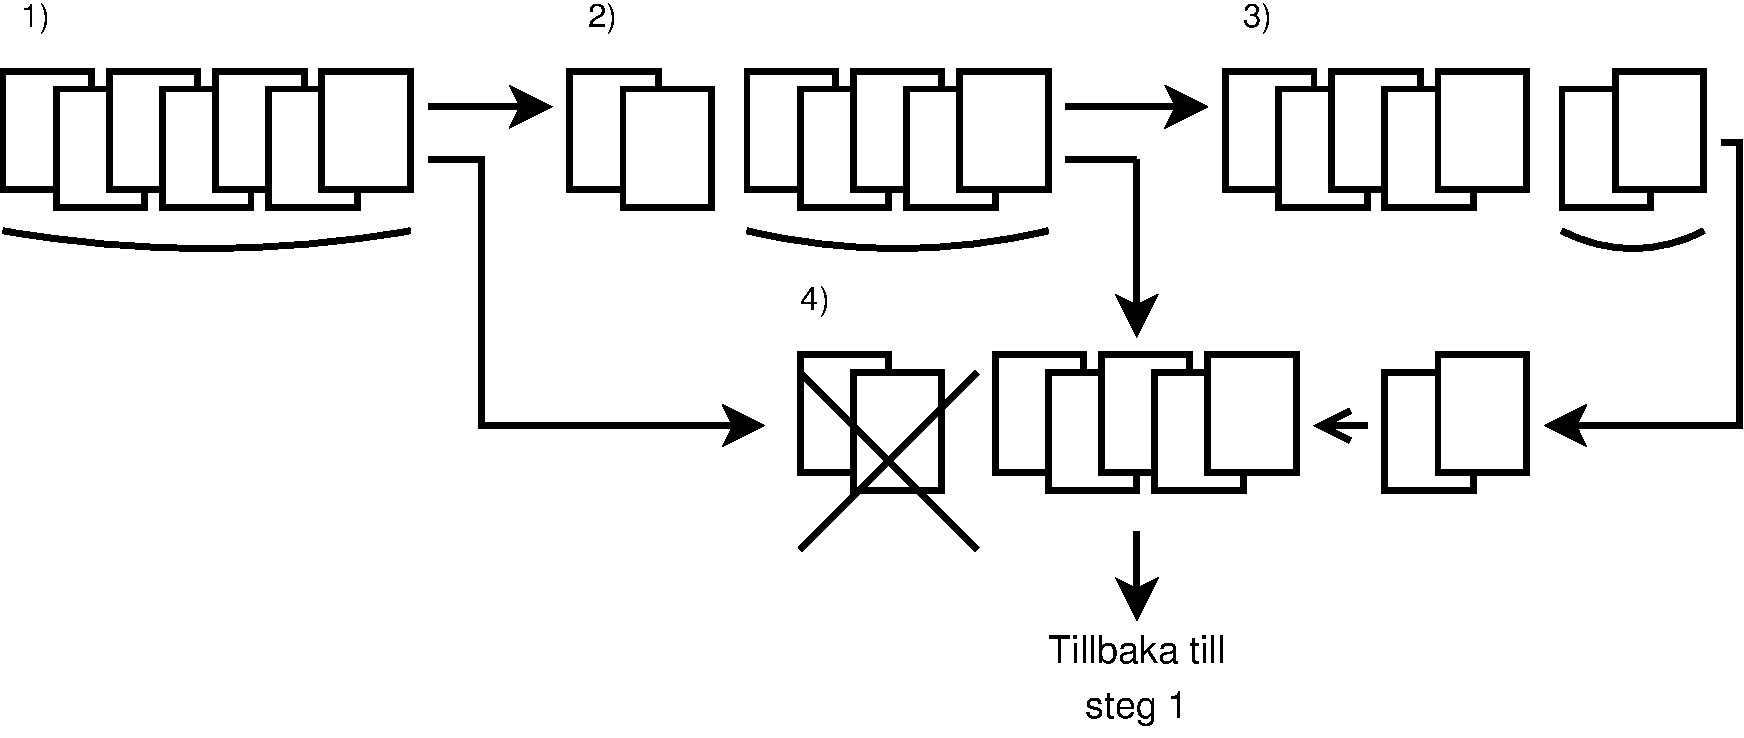
\includegraphics[width=0.95\textwidth]{bilder/HMM_flowchart}
  \caption[Klassificering av dynamiska gester med två, fem och sju
  symboler]{Klassificering av dynamiska gester med två, fem och sju
  symboler sker enligt en relativt enkel procedur:
  \begin{enumerate}
    \item Programmet beräknar sannolikheten att en HMM tränad med sju
	symboler skapat symbolföljden. Är någon sannolikhet tillräckligt hög 
	registreras den aktuella gesten och programmet går till steg fyra, 
	annars går det vidare till steg två.
    \item Programmet beräknar sannolikheten att de fem senaste symbolerna
	skapats av en HMM tränad med fem symboler. Vid tillräckligt hög sannolikhet 
	registreras en gest och programmet går till steg fyra, annars går det 
	vidare till steg tre. 
    \item Programmet beräknar sannolikheten att de två senaste symbolerna skapats av 
	en HMM tränad med två symboler. Om sannolikheten är tillräckligt hög registreras
	en (statisk) gest. 
    \item De två äldsta symbolerna kasseras och två nya sätts in i slutet av följden. 
	Programmet börjar om från steg ett.
  \end{enumerate}
	 Märk att denna algoritm prioriterar långa symbolföljder,
	d.v.s.~störst går först.}
  \label{fig:hmm-flowchart}
\end{figure}
 
 \end{document}

